% Chapter Template

\chapter{An approach to VAD using PEFAC} % Main chapter title

\label{Chapter5} % Change X to a consecutive number; for referencing this chapter elsewhere, use \ref{ChapterX}

\lhead{Chapter 5. \emph{An approach to VAD using PEFAC}} % Change X to a consecutive number; this is for the header on each page - perhaps a shortened title

%----------------------------------------------------------------------------------------
%	SECTION 1 - PEFAC pitch tracker
%----------------------------------------------------------------------------------------

\section{PEFAC pitch tracker}

PEFAC pitch tracker \cite{PEFAC} is one of the recently published, robust pitch tracking algorithms which has been reported to achieve good results even at negative signal to noise ratios. Apart from calculating the pitch estimate as its primary output, it has also been designed to estimate the probability of a given frame \emph{being voiced} which is essentially a voiced speech activity detector. This value can be used to detect the voiced parts of a speech utterance by simple thresholding. Subsequent application of a hang-over scheme from Chapter \ref{Chapter3} should help in detecting the unvoiced segments. A combination of a thresholding stage and the hang-over scheme therefore creates a complete Voice Activity Detector.

The rest of this chapter is organised as follows. Firstly, an overview of PEFAC is presented. Then, the proposed approach to VAD is described in more detail, implemented and evaluated against LTSD, which was the best performing VAD from Chapter \ref{Chapter4}. The experimental set-up for evaluation of PEFAC as VAD is the same as described in Chapter \ref{Chapter3}.

%----------------------------------------------------------------------------------------
%	SUBSECTION 1 - PEFAC algorithm description
%----------------------------------------------------------------------------------------

\subsection{PEFAC algorithm description}

A detailed description of PEFAC is available in \cite{PEFAC}. The algorithm can however be summarised in the following steps:
\begin{enumerate}
\item Transform the input signal to the power spectrum domain using short-time Fourier transform
\item Interpolate the periodogram of each frame onto a log-spaced frequency grid
\item Calculate the normalized periodogram
\item Convolve the normalized periodogram with a comb filter in order to enhance speech harmonics and attenuate the noise
\item Select the three highest peaks in the feasible range as the initial pitch candidates
\item Estimate the probability of a frame being voiced
\item Use dynamic programming to identify the final pitch estimate
\end{enumerate}

The probability of a frame being voiced is based on two features:
\begin{enumerate}
\item The log-mean power of a frame $L_t = \log E_t$ such that $E_t = \frac{1}{Q} \sum_{n=1}^{Q} Y_t(q_i)$ where $Q$ is the number of frequency bins, $Y_t(q)$ is the normalized log-frequency periodogram. Using the log-mean power is justified since voiced speech typically contains most energy from a complete speech utterance and its mean power is therefore higher than that of unvoiced speech
\item The ratio of the sum of the highest three peaks in the spectrum convolved with the comb filter to $E_t$. Voiced speech contains most of its power in the harmonic bins therefore using this measure as a second feature is justified
\end{enumerate}

%----------------------------------------------------------------------------------------
%	SECTION 2
%----------------------------------------------------------------------------------------

\section{The proposed approach}

The proposed approach is relatively simple. PEFAC returns the probability of the current frame being voiced in a typical manner, i.e. as a number in the range 0 to 1. This can easily be thresholded and the voiced frames can be identified at this step. As stated numerously in the previous chapters, voiced frames are typically surrounded by unvoiced ones, hence application of the hang-over scheme from Section \ref{sec:hang} should help to detect them. Overall, this approach should perform well in detection of both voiced as well as unvoiced phonemes which is the aim of a complete Voice Activity Detector.

%----------------------------------------------------------------------------------------
%	SECTION 3 - Evaluation results
%----------------------------------------------------------------------------------------

\section{Evaluation results}

The proposed approach has been implemented, evaluated and compared with the LTSD VAD. In all experiments, the hang-over scheme (Section \ref{sec:hang}) has been applied to both algorithms. The evaluation of PEFAC without it does not make much sense, since by design it does not detect unvoiced phonemes and they need to be identified by a secondary method. Other than that, the evaluation metrics are the same as in Chapter \ref{Chapter4}, namely the ROC curves and speech/non-speech hit rates with a fixed threshold.

%----------------------------------------------------------------------------------------
%	SUBSECTION 1 - ROC curves
%----------------------------------------------------------------------------------------

\subsection{ROC curves}

The ROC curves for PEFAC and LTSD for all six noise types and two SNRs (-5 dB and -10 dB) are presented in Figures \ref{fig:pefacm5} and \ref{fig:pefacm10}. For the white, car and opsroom noises, the performance of both algorithms seems to be comparable. In the white noise, PEFAC's performance drops more quickly as the threshold value increases\footnote{For an extreme threshold value of 0, all frames would be classified as speech hence it represents the (1,1) point on the plot.}, however the point at which the curve bends down is achieved at a smaller false positive rate than in case of LTSD. The same applies to the car noise. PEFAC clearly underperforms LTSD in the babble and spchspect noises, which is expected to some extent, since being primarily a pitch tracker, the babble noise is probably the most difficult noise in which such algorithm might operate. What is promising however is that PEFAC is far superior to LTSD in the factory noise and its performance is much better in both SNRs.

\begin{figure}[htbp]
	\centering
		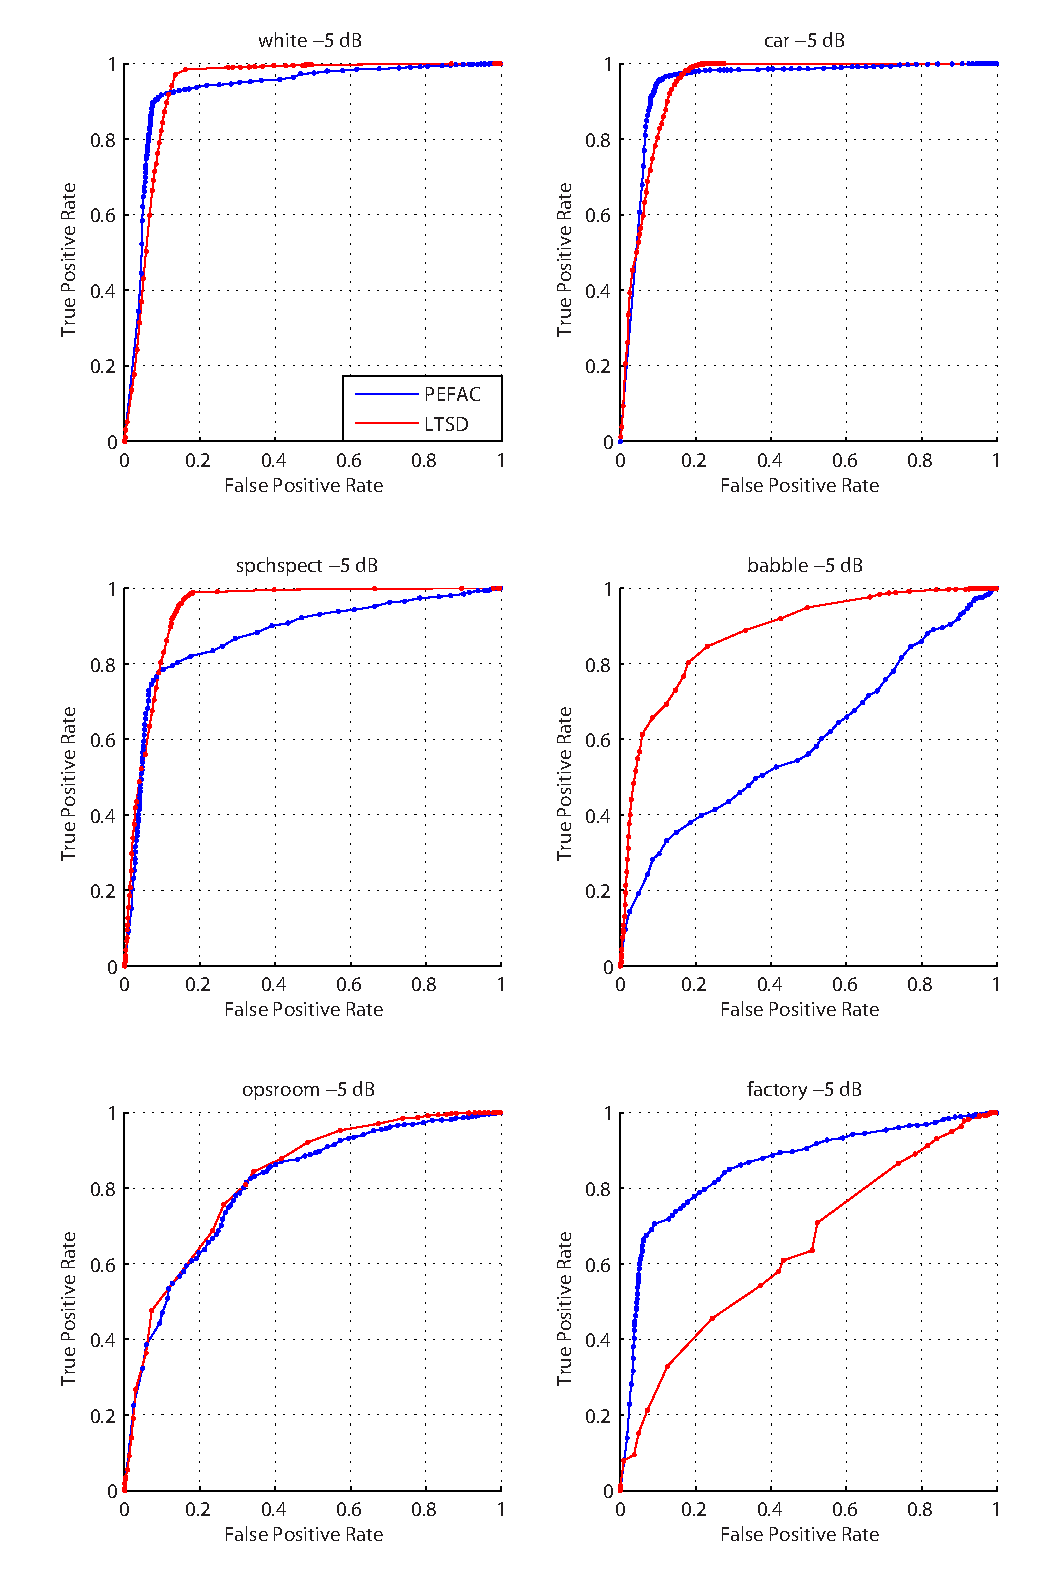
\includegraphics[width=1.0\columnwidth]{Figures/Chapter5/pefacm5.pdf}
		\rule{37em}{0.5pt}
	\caption[ROC curves of PEFAC and LTSD \emph{with} hang-over under -5 dB SNR]{ROC curves of PEFAC and LTSD \emph{with} hang-over under -5 dB SNR}
	\label{fig:pefacm5}
\end{figure}

\begin{figure}[htbp]
	\centering
		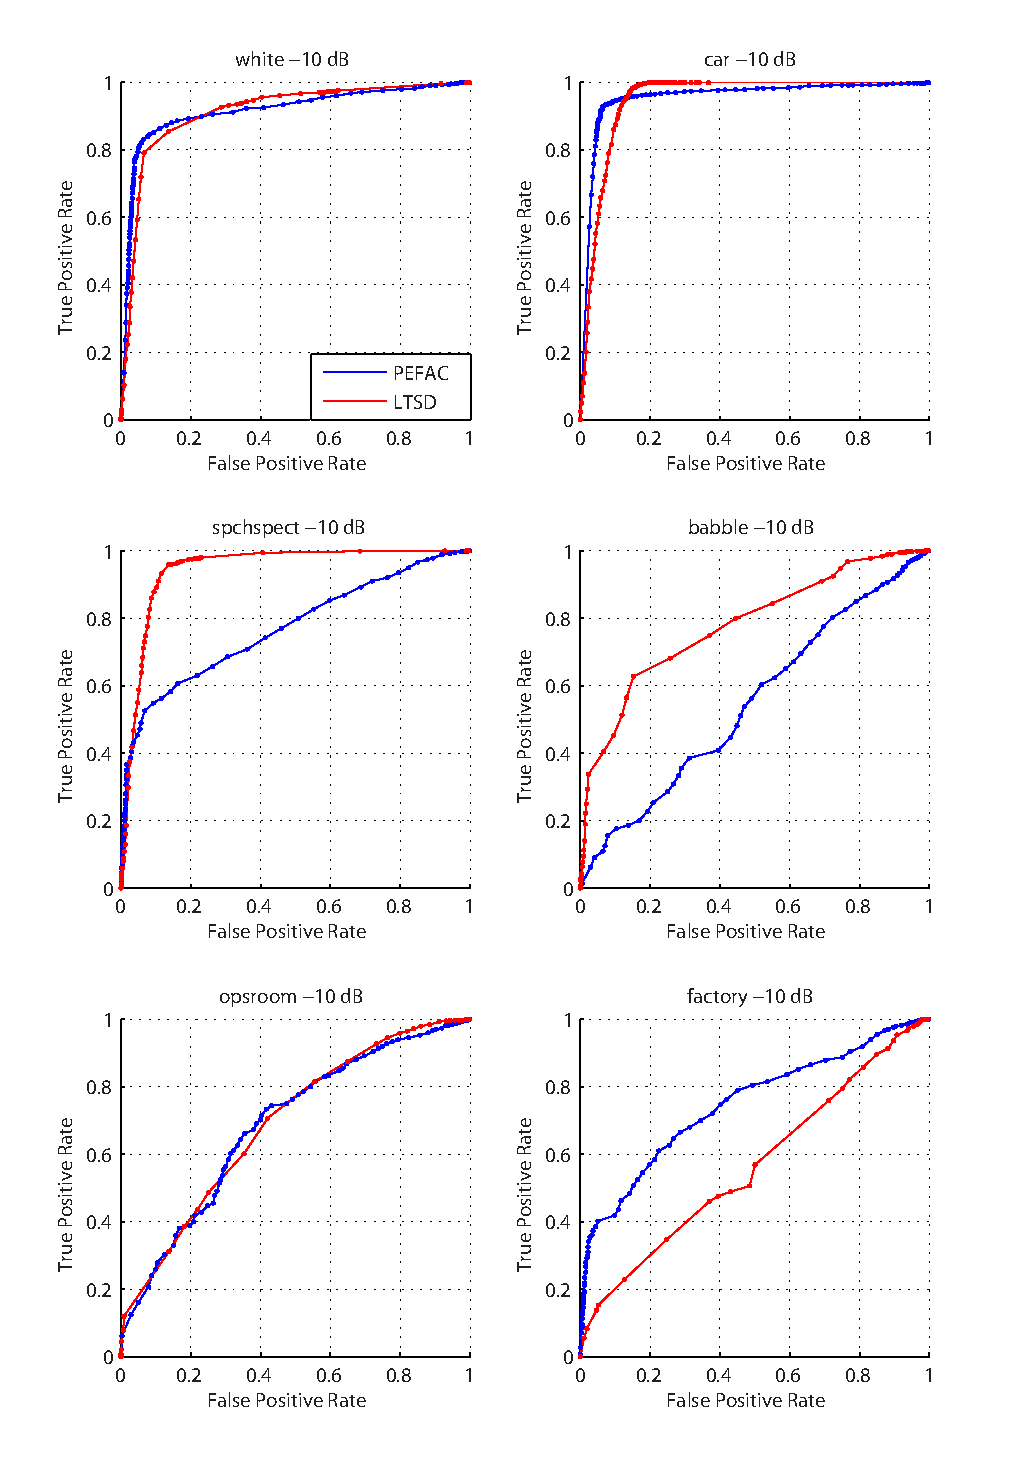
\includegraphics[width=1.0\columnwidth]{Figures/Chapter5/pefacm10.pdf}
		\rule{37em}{0.5pt}
	\caption[ROC curves of PEFAC and LTSD \emph{with} hang-over under -10 dB SNR]{ROC curves of PEFAC and LTSD \emph{with} hang-over under -10 dB SNR}
	\label{fig:pefacm10}
\end{figure}

%----------------------------------------------------------------------------------------
%	SUBSECTION 2 - Speech/non-speech hit rates
%----------------------------------------------------------------------------------------

\subsection{Speech/non-speech hit rates}

The speech/non-speech hit rates with two fixed thresholds (0.60 and 0.55 respectively) are presented in Figures \ref{fig:pefacSNR60} and \ref{fig:pefacSNR55}\footnote{The threshold for PEFAC in Figure \ref{fig:pefacSNR60} is higher than in \ref{fig:pefacSNR55} therefore a lower speech hit rate but a higher non-speech hit rate. The thresholds are 0.60 and 0.55 respectively.}. Interestingly, for both threshold values PEFAC overperforms LTSD at low and very low SNRs i.e. in the range 0 to -15 dB. For the higher value of the fixed threshold (Figure \ref{fig:pefacSNR60}) PEFAC's performance is clearly better even in both speech and non-speech metrics while for the lower threshold, the non-speech hit rate at the low SNRs is very similar for both algorithms.

\begin{figure}[htbp]
	\centering
		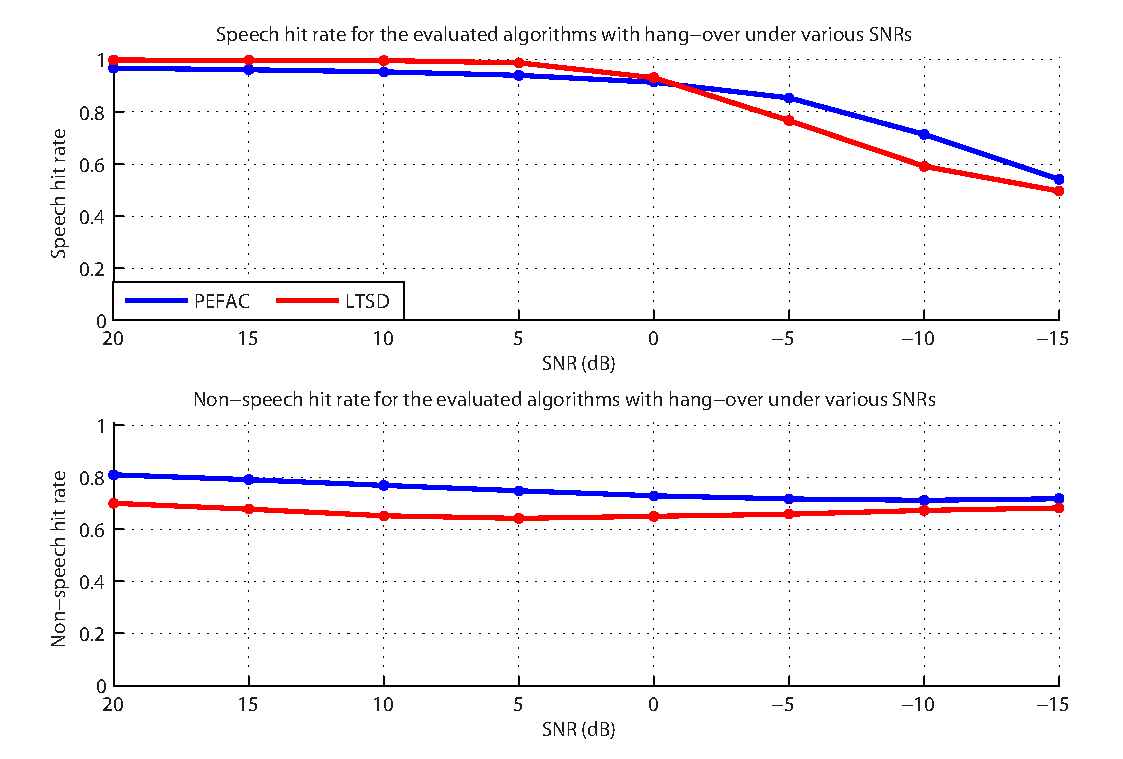
\includegraphics[width=0.9\columnwidth]{Figures/Chapter5/pefacSNR60bold.pdf}
		\rule{37em}{0.5pt}
	\caption[Speech/non-speech hit rates of PEFAC (threshold 0.60) and LTSD under different SNRs]{Speech/non-speech hit rates of PEFAC (threshold 0.60) and LTSD under different SNRs}
	\label{fig:pefacSNR60}
\end{figure}

\begin{figure}[htbp]
	\centering
		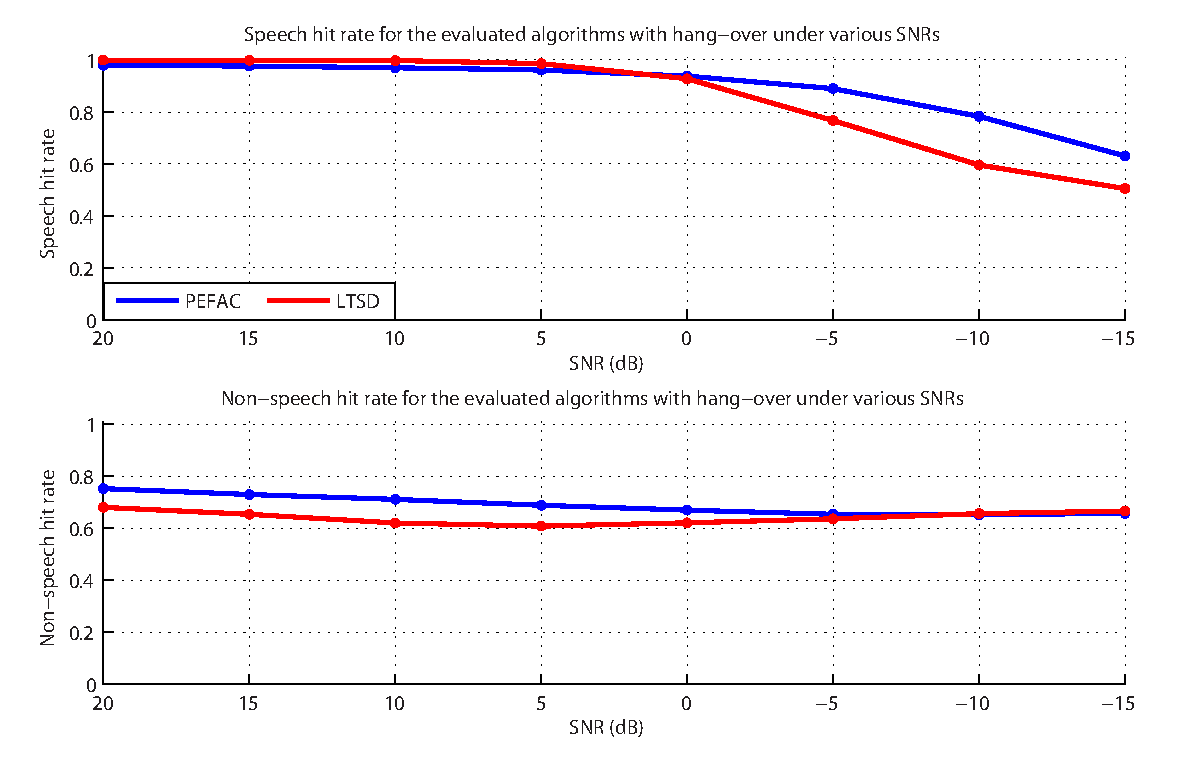
\includegraphics[width=0.9\columnwidth]{Figures/Chapter5/pefacSNR55bold.pdf}
		\rule{37em}{0.5pt}
	\caption[Speech/non-speech hit rates of PEFAC (threshold 0.55) and LTSD under different SNRs]{Speech/non-speech hit rates of PEFAC (threshold 0.55) and LTSD under different SNRs}
	\label{fig:pefacSNR55}
\end{figure}

\clearpage

%----------------------------------------------------------------------------------------
%	SECTION 4 - Impact of hang-over parameters
%----------------------------------------------------------------------------------------

\section{Impact of hang-over parameters}

There is a slight disadvantage in the performance of PEFAC in the speech hit rate at the high SNRs (20 dB to 5 dB). The position of the speech classified as noise errors (i.e. false negatives) has initially been investigated visually by examining plots of the test set overlaid with the reference labels and VAD decisions. It has been determined that the vast majority of PEFAC's speech classified as noise errors appear at the very endings of the utterances. This is visualised in Figure \ref{fig:clipping} where such errors are labelled as BEC - back end clipping. The errors which do appear are very short, the length of which is around 1-2 frames and hence can be described as minor. There are virtually no MSC (midspeech clipping) errors, which are more severe, for both LTSD and PEFAC at high SNRs and only a small number of FEC (front end clipping) errors.

On the other hand, if an entire utterance is classified correctly, the labels returned by both PEFAC and LTSD are often wider than the reference and tend to capture the utterance together with some of the noise frames surrounding the beginning and ending of it. This types of errors are not very serious and a more detailed analysis of them is described in the next section. 

\begin{figure}[htbp]
	\centering
		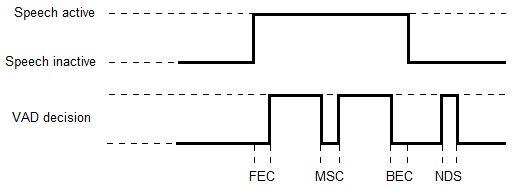
\includegraphics[width=1.0\columnwidth]{Figures/Chapter5/clipping.png}
		\rule{37em}{0.5pt}
	\caption[Types of misclassifications in VAD]{Types of misclassifications in VAD. FEC - front end clipping, MSC - midspeech clipping, BEC - back end clipping, NDS - noise detected as speech}
	\label{fig:clipping}
\end{figure}

The fact that most speech false negatives are BEC errors indicates a hypothesis that the differences in the performance of both algorithms at the high SNRs could be reduced by careful calibration of the hang-over parameters and the frame length. In particular, the parameters $L_s$ and $L_m$, as in Algorithm \ref{algo:hangover} with which the previous evaluation has been performed are not large enough to extend the initial VAD decisions to capture all beginnings and endings of the speech utterances. In order to confirm the hypothesis, an experimentation with various different parameter values has been performed and the speech/non-speech hit rates have been examined. It transpired that by reducing the frame length\footnote{The frame length has been reduced from 50 ms to 25 ms.} and adjusting the other parameters appropriately\footnote{The new parameter values are $B=14$, $S_p=3$, $S_l=5$, $L_s=18$ and $L_m=25$.}, the performance of both algorithms can be rendered almost equal at the high SNRs with PEFAC still outperforming LTSD at the low SNRs. Figure \ref{fig:diffhangpars} presents the result of the new evaluation.

\begin{figure}[htbp]
	\centering
		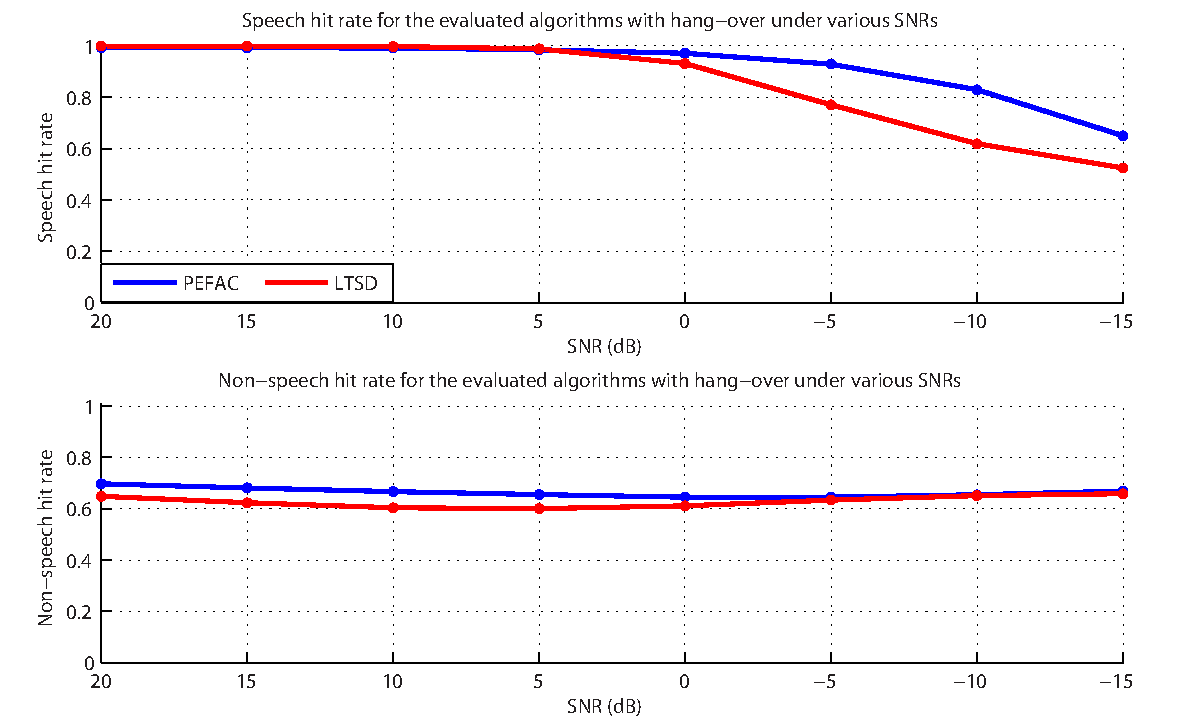
\includegraphics[width=0.9\columnwidth]{Figures/Chapter5/diffhangpars.pdf}
		\rule{37em}{0.5pt}
	\caption[Speech/non-speech hit rates of PEFAC (threshold 0.60) and LTSD with adjusted hang-over parameters]{Speech/non-speech hit rates of PEFAC (threshold 0.60) and LTSD with adjusted hang-over parameters}
	\label{fig:diffhangpars}
\end{figure}

%----------------------------------------------------------------------------------------
%	SECTION 5 - Position of false positives
%----------------------------------------------------------------------------------------

\section{Position of false positives}

While at the high SNRs the detection of speech frames is almost perfect, there is still around 35\% misclassification rate of the noise frames. However, it can be argued that the seriousness of errors which appear at different places in the recording is not the same. In particular, a noise as speech error (i.e. false positive) appearing in vicinity of an actual speech is not as disadvantageous as the same error in the middle of a long noise-only period. In order to identify what is the distribution of the distances between a misclassified noise to the nearest speech, histograms of them at various SNRs have been generated and are presented in Figure \ref{fig:histSpch}.

Analysis of the histograms shows that most errors at high SNRs for both algorithms appear close to actual speech utterances. In particular, at 20 dB more than 50\% of the errors in both algorithms appear no further than half a second from an actual speech frame. For LTSD, this value holds even at 0 dB. As already mentioned in the previous section, whenever any of the algorithms identifies a speech segment it tends to overstretch the speech labels insignificantly in front of the beginning and beyond the ending of the utterance. However, given that the reference labels have been designed to have a very sharp cut-off (Figure \ref{fig:groundtruth}) it might be concluded that such errors are of a very minor nature. In fact, such segments before and after an utterance could be given a \emph{don't care} label (as briefly discussed in Section \ref{sec:speechlabels}) and then such VAD decisions would not even be treated as errors at all. Additionally, as the SNR becomes lower, the distribution of errors becomes smoother. This is is unsurprising because as the SNR conditions deteriorate, both algorithms tend to make a higher number of random errors in the middle of noise-only periods.

\begin{figure}[htbp]
	\centering
		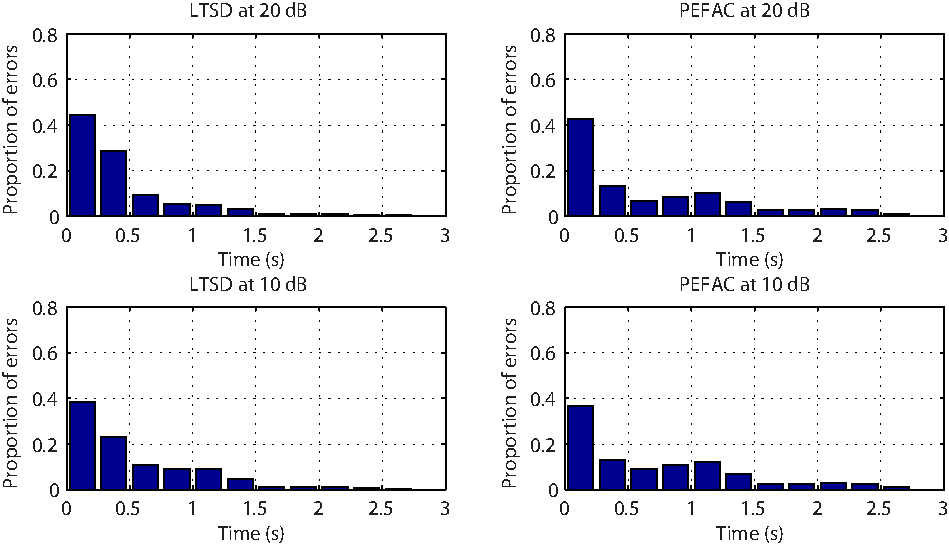
\includegraphics[width=1.0\columnwidth]{Figures/Chapter5/histSpch20dB10dB.pdf}
		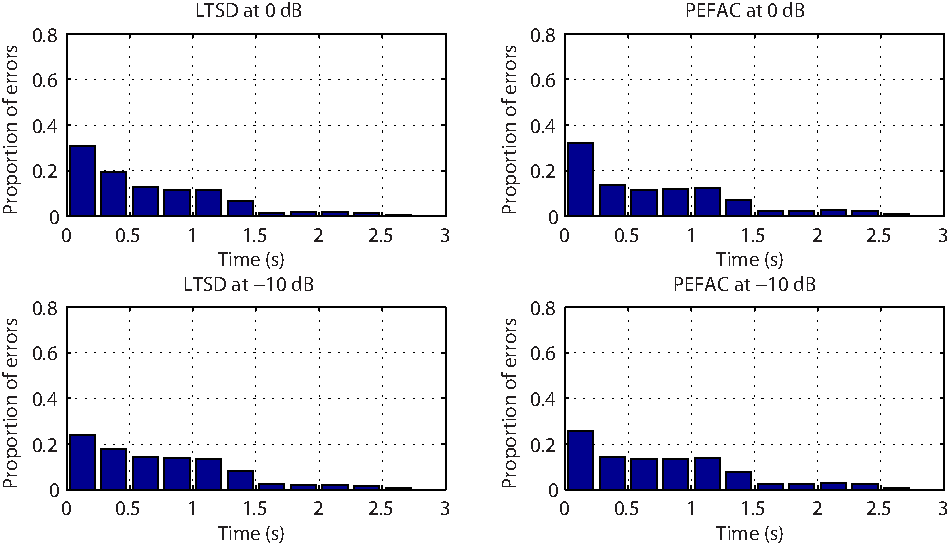
\includegraphics[width=1.0\columnwidth]{Figures/Chapter5/histSpch0dBm10dB.pdf}
		\rule{37em}{0.5pt}
	\caption[Histograms of the distances between a false positive error and the nearest true positive]{Histograms of the distances between a false positive error and the nearest true positive}
	\label{fig:histSpch}
\end{figure}

%----------------------------------------------------------------------------------------
%	SECTION 6 - Position of false negatives
%----------------------------------------------------------------------------------------

\section{Position of false negatives}

A similar analysis can be performed for speech classified as noise errors and the histograms for 10 dB, 0 dB and -10 dB are presented in Figure \ref{fig:histNoi}. Under 20 dB SNR there are virtually no false negatives returned by any of the algorithms hence a histogram for this SNR has not been generated. Similarly to the previous section, at high SNR most false negatives appear close to actual noise frames (i.e. an actual noise frame is not futher than 0.25 seconds from the error). This types of misclassifications are either FEC or BEC errors (Figure \ref{fig:clipping}) and might be tolerable in some applications. Despite that, the main aim of a VAD system is to detect all speech segments and hence all other errors should not appear at all.

For PEFAC, there is a strange spike in the proportion of errors appearing between 1.25 and 1.75 seconds from an actual noise frame at 10 dB and 0 dB however it is unclear why such phenomenon occurs. Similarly to the false positives, the distribution of errors becomes smoother with falling SNR.

\begin{figure}[htbp]
	\centering
		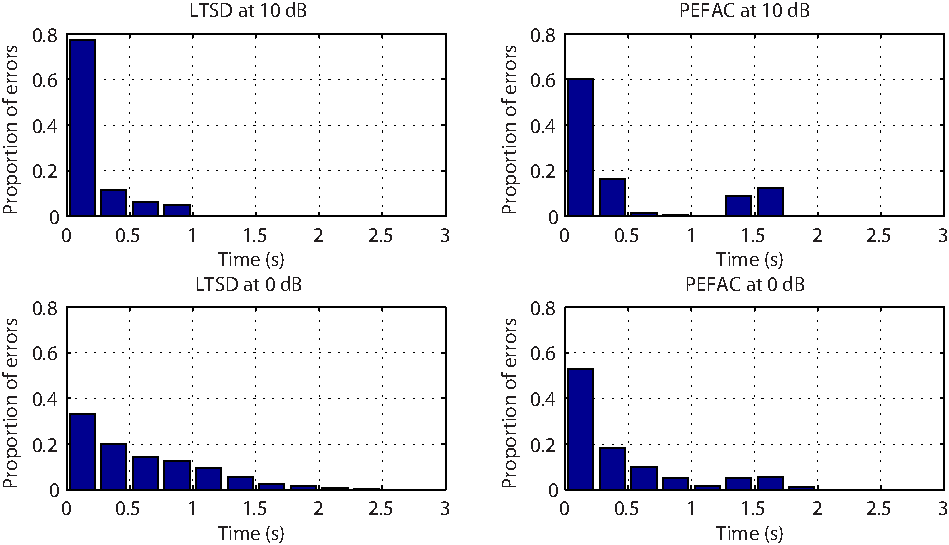
\includegraphics[width=1.0\columnwidth]{Figures/Chapter5/histNoi10dB0dB.pdf}
		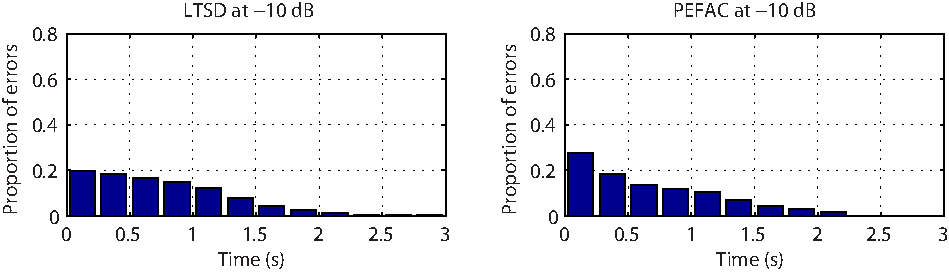
\includegraphics[width=1.0\columnwidth]{Figures/Chapter5/histNoim10dB.pdf}
		\rule{37em}{0.5pt}
	\caption[Histograms of the distances between a false negative error and the nearest true negative]{Histograms of the distances between a false negative error and the nearest true negative}
	\label{fig:histNoi}
\end{figure}

%----------------------------------------------------------------------------------------
%	SECTION 6 - Summary
%----------------------------------------------------------------------------------------

\section{Conclusion}

The overall performance of PEFAC is better than LTSD's at the very low SNRs (0 dB to -15 dB). This performance gain comes mostly from the much better operation in the factory noise and the fact that the best performance of PEFAC in all six noise types is achieved at similar threshold values (around 0.6) while for the LTSD algorithm the threshold values vary significantly between different noise types. Despite better performance in the speech/non-speech hit rates, the false positives returned by PEFAC seem to be a little more serious than LTSD's as determined by the distance between the false positive and the nearest true positive.

Overall it can be said that LTSD is a preferable algorithm for applications which operate predominantly in noise conditions which are known beforehand or the SNR is very high, i.e. greater than 10 dB. This conclusion is drawn from Figures \ref{fig:pefacm5} and \ref{fig:pefacm10} where for most noise types it is often possible to determine a value for the LTSD's threshold such that it will outperform PEFAC in this particular noise type and SNR (with exemption of the factory noise).

PEFAC on the other hand should be considered for applications which suffer from a variety of changing noise types or low SNRs. This is confirmed by Figure \ref{fig:diffhangpars} where PEFAC outperforms LTSD significantly at the very low SNRs. For such conditions, the performance is still not perfect, as the speech hit-rate is well below 100\%, however with a precise adjustment of the threshold value and/or the hang-over parameters it should be possible to raise it to a satisfactory level. However, the main disadvantage of such approach would be an algorithm whose good performance is limited to a small number of environments.